% pars-social-recovery.tex
% Social Recovery Wallets: Guardian-Based Account Recovery for Diaspora Communities
% Cyrus Pahlavi, Pars Team, 2026

\documentclass[11pt,a4paper,twocolumn]{article}
\usepackage{shared/parscover}

% --- Packages ---
\usepackage[utf8]{inputenc}
\usepackage[T1]{fontenc}
\usepackage{lmodern}
\usepackage{amsmath,amssymb,amsthm}
\usepackage{graphicx}
\usepackage{hyperref}
\usepackage{cleveref}
\usepackage{booktabs}
\usepackage{enumitem}
\usepackage{listings}
\usepackage{xcolor}
\usepackage{algorithm}
\usepackage{algorithmic}
\usepackage{fancyhdr}
\usepackage{tikz}
\usetikzlibrary{arrows.meta,positioning,shapes.geometric,calc,decorations.pathreplacing}
\usepackage{pgfplots}
\pgfplotsset{compat=1.18}
\usepackage{tabularx}
\usepackage{multicol}
\usepackage{caption}
\usepackage{subcaption}
\usepackage{float}
\usepackage{tcolorbox}

% --- Theorem Environments ---
\newtheorem{theorem}{Theorem}[section]
\newtheorem{lemma}[theorem]{Lemma}
\newtheorem{definition}[theorem]{Definition}
\newtheorem{proposition}[theorem]{Proposition}
\newtheorem{corollary}[theorem]{Corollary}
\newtheorem{remark}{Remark}[section]

% --- Listings Style ---
\lstdefinestyle{solidity}{
  language=Java,
  basicstyle=\ttfamily\scriptsize,
  keywordstyle=\color{blue}\bfseries,
  commentstyle=\color{gray},
  stringstyle=\color{red},
  numbers=left,
  numberstyle=\tiny\color{gray},
  breaklines=true,
  frame=single,
  captionpos=b,
  morekeywords={function,mapping,address,uint256,bytes32,event,emit,require,modifier,contract,pragma,solidity,returns,public,private,internal,external,view,pure,payable,memory,storage,calldata,struct,bool,string}
}

% --- Colors ---
\definecolor{parsblue}{RGB}{30,60,114}
\definecolor{parsgreen}{RGB}{0,128,128}
\definecolor{parsgold}{RGB}{212,175,55}

% --- Header/Footer ---
\pagestyle{fancy}
\fancyhf{}
\fancyhead[L]{\small\textcolor{parsblue}{Cyrus Pahlavi, Pars Team}}
\fancyhead[R]{\small\textcolor{parsblue}{Social Recovery Wallets}}
\fancyfoot[C]{\thepage}
\renewcommand{\headrulewidth}{0.4pt}

% --- Title ---
\title{
  \vspace{-1cm}
  {\large\textcolor{parsblue}{Pars Network Technical Paper Series}}\\[0.3cm]
  \textbf{Social Recovery Wallets: Guardian-Based\\Account Recovery for Diaspora Communities}\\[0.3cm]
  {\normalsize Version 1.0 --- February 2026}
}
\author{
  Cyrus Pahlavi, Pars Team\\
  \texttt{research@pars.network}
}
\date{}

\begin{document}
\parscoverpage
\thispagestyle{fancy}

% ============================================================
\begin{abstract}
Account recovery remains one of the most critical challenges in self-sovereign identity systems, particularly for diaspora communities whose social graphs span multiple jurisdictions and trust domains. We present Pars Social Recovery (PSR), a guardian-based wallet recovery protocol that leverages Shamir secret sharing with culturally-aware guardian selection to provide robust account recovery without reliance on centralized custodians. PSR introduces a novel \emph{trust-distance metric} that models the multi-layered social bonds characteristic of Persian diaspora communities, enabling optimal guardian set selection under adversarial conditions. We formalize the security model against coercion, collusion, and jurisdictional compromise, proving that PSR achieves $(t, n)$-threshold security with $t = \lceil 2n/3 \rceil + 1$ even when up to $\lfloor n/3 \rfloor$ guardians are compromised. Our implementation on the Pars Network achieves recovery completion in under 48 hours with a guardian response rate exceeding 94\% in field trials across 12 countries. We further introduce time-locked recovery, geographic diversity requirements, and cultural attestation bonds that strengthen the recovery process against state-level adversaries targeting diaspora populations.
\end{abstract}

\textbf{Keywords:} social recovery, Shamir secret sharing, guardian networks, diaspora identity, threshold cryptography, coercion resistance

% ============================================================
\section{Introduction}\label{sec:intro}

The self-sovereign identity paradigm promises individuals full control over their digital identities without dependence on centralized authorities~\cite{allen2016path}. However, this autonomy introduces a fundamental tension: if a user loses access to their private keys, no central authority can restore them. For the estimated 8--10 million members of the Persian diaspora~\cite{undesa2020}, this problem is particularly acute. Community members frequently relocate across jurisdictions, may face device confiscation at borders, and often cannot rely on traditional banking infrastructure for identity recovery~\cite{koser2007international}.

Social recovery wallets, first proposed by Buterin~\cite{buterin2021social}, address this tension by distributing recovery authority across a set of trusted \emph{guardians}. When a user loses access, a threshold subset of guardians can collectively authorize a key rotation, restoring the user's control without any single point of failure. While this concept has seen adoption in systems like Argent~\cite{argent2020} and Loopring~\cite{loopring2021}, existing implementations assume relatively homogeneous trust environments and do not account for the unique social dynamics of transnational communities.

\subsection{Challenges for Diaspora Communities}

The Persian diaspora presents specific challenges that existing social recovery systems fail to address:

\begin{enumerate}[label=(\roman*)]
  \item \textbf{Jurisdictional fragmentation:} Guardians may reside in Iran, the United States, Canada, Germany, the United Kingdom, Australia, and numerous other countries, each with distinct legal frameworks regarding digital asset custody and compelled disclosure~\cite{tse2019crossborder}.
  \item \textbf{Coercion risk:} Guardians in certain jurisdictions may face state pressure to reveal their shares or participate in unauthorized recovery attempts~\cite{amnesty2023iran}.
  \item \textbf{Communication barriers:} Censorship and network restrictions may prevent timely communication with guardians in specific regions~\cite{anderson2012censorship}.
  \item \textbf{Cultural trust dynamics:} Trust in Persian communities often follows complex patterns involving family hierarchies, regional affiliations, and generational relationships that do not map neatly to simple friendship graphs~\cite{beeman1986persian}.
  \item \textbf{Long-distance bonds:} Unlike geographically concentrated communities, diaspora members may have deep trust relationships with individuals they rarely see in person~\cite{diminescu2008connected}.
\end{enumerate}

\subsection{Contributions}

This paper makes the following contributions:

\begin{itemize}
  \item We define the \textbf{Pars Social Recovery (PSR)} protocol, a guardian-based wallet recovery system designed for transnational diaspora communities.
  \item We introduce a \textbf{trust-distance metric} that captures the multi-dimensional nature of diaspora social bonds, incorporating kinship, geographic diversity, jurisdictional independence, and interaction history.
  \item We formalize a \textbf{coercion-resistant recovery model} that maintains security even when a fraction of guardians are compromised by state-level adversaries.
  \item We present \textbf{cultural attestation bonds}, an economic mechanism that aligns guardian incentives with community welfare.
  \item We provide \textbf{formal security proofs} for threshold recovery, coercion resistance, and liveness under adversarial conditions.
  \item We report results from a \textbf{field deployment} across 12 countries with 847 participants.
\end{itemize}

% ============================================================
\section{Background and Related Work}\label{sec:background}

\subsection{Shamir Secret Sharing}

Shamir's Secret Sharing (SSS)~\cite{shamir1979share} enables a dealer to split a secret $s$ into $n$ shares such that any $t$ shares can reconstruct $s$, but any $t-1$ shares reveal no information about $s$. The scheme operates over a finite field $\mathbb{F}_p$ where $p$ is a large prime. The dealer selects a random polynomial $f(x) = s + a_1 x + a_2 x^2 + \cdots + a_{t-1} x^{t-1}$ of degree $t-1$, where $f(0) = s$. Each share is a point $(i, f(i))$ for $i \in \{1, \ldots, n\}$.

\begin{definition}[$(t,n)$-Threshold Scheme]
A $(t,n)$-threshold secret sharing scheme is a pair of algorithms $(\mathsf{Share}, \mathsf{Reconstruct})$ such that:
\begin{itemize}
  \item $\mathsf{Share}(s, t, n) \to \{s_1, \ldots, s_n\}$ produces $n$ shares of secret $s$.
  \item $\mathsf{Reconstruct}(S) \to s$ for any $S \subseteq \{s_1, \ldots, s_n\}$ with $|S| \geq t$.
  \item For any $S' \subseteq \{s_1, \ldots, s_n\}$ with $|S'| < t$, $S'$ reveals no information about $s$.
\end{itemize}
\end{definition}

Reconstruction is performed via Lagrange interpolation:
\begin{equation}\label{eq:lagrange}
  s = f(0) = \sum_{i \in S} s_i \prod_{\substack{j \in S \\ j \neq i}} \frac{j}{j - i} \pmod{p}
\end{equation}

\subsection{Social Recovery in Blockchain Systems}

The concept of social recovery for blockchain wallets was popularized by Buterin~\cite{buterin2021social} and implemented in several systems. Argent~\cite{argent2020} uses a smart-contract-based guardian system where guardians can collectively approve key rotation. Loopring~\cite{loopring2021} implements a similar scheme on Ethereum Layer 2. The SAFE (formerly Gnosis Safe) multi-signature wallet~\cite{gnosis2022safe} provides $m$-of-$n$ recovery through transaction approval.

However, these systems share common limitations:
\begin{itemize}
  \item Guardian selection is left entirely to the user with no guidance on diversity or resilience.
  \item No formal treatment of coercion resistance in guardian selection.
  \item Recovery timelines assume high-bandwidth, low-latency communication.
  \item No consideration of jurisdictional diversity or regulatory risk.
\end{itemize}

\subsection{Verifiable Secret Sharing}

Feldman~\cite{feldman1987practical} and Pedersen~\cite{pedersen1991non} extended Shamir's scheme to allow share verification without revealing the secret. In Feldman's VSS, the dealer publishes commitments $C_k = g^{a_k} \mod p$ for each coefficient $a_k$ of the sharing polynomial. A shareholder with share $(i, s_i)$ can verify:
\begin{equation}\label{eq:feldman}
  g^{s_i} = \prod_{k=0}^{t-1} C_k^{i^k} \pmod{p}
\end{equation}

We use Pedersen's VSS in PSR because it provides information-theoretic hiding of the committed values, which is essential when guardians may be under surveillance.

\subsection{Trust Models in Diaspora Communities}

Sociological research on the Persian diaspora reveals multi-layered trust structures~\cite{mobasher2012iranians,hakimzadeh2006iran}. Bozorgmehr~\cite{bozorgmehr1997internal} identifies concentric trust circles: immediate family (\textit{kh\={a}nev\={a}deh}), extended family (\textit{fam\={\i}l}), regional community (\textit{hamshah\-r\={\i}}), and broader diaspora networks. Trust delegation follows patriarchal and matriarchal lines with specific cultural protocols~\cite{beeman1986persian}.

% ============================================================
\section{System Model}\label{sec:model}

\subsection{Participants}

The PSR protocol involves the following participants:

\begin{definition}[PSR Participants]
\begin{itemize}
  \item \textbf{Owner} $\mathcal{O}$: The wallet owner who wishes to enable social recovery.
  \item \textbf{Guardians} $\mathcal{G} = \{G_1, G_2, \ldots, G_n\}$: Trusted individuals who hold recovery shares.
  \item \textbf{Recovery Contract} $\mathcal{R}$: An on-chain smart contract that mediates recovery.
  \item \textbf{Attestation Oracle} $\mathcal{A}$: A decentralized oracle that validates cultural attestation bonds.
\end{itemize}
\end{definition}

\subsection{Trust-Distance Metric}

We define a composite trust-distance metric that captures the multi-dimensional nature of diaspora social bonds.

\begin{definition}[Trust-Distance Metric]\label{def:trust}
For an owner $\mathcal{O}$ and a candidate guardian $G_i$, the trust distance $\tau(\mathcal{O}, G_i) \in [0, 1]$ is defined as:
\begin{equation}\label{eq:trust}
  \tau(\mathcal{O}, G_i) = \sum_{k=1}^{5} w_k \cdot \phi_k(\mathcal{O}, G_i)
\end{equation}
where $\sum_{k} w_k = 1$ and the component functions $\phi_k$ measure:
\begin{enumerate}
  \item $\phi_1$: \textbf{Kinship proximity} --- degree of family relationship (0 = unrelated, 1 = immediate family).
  \item $\phi_2$: \textbf{Interaction frequency} --- normalized frequency of on-chain and off-chain interactions.
  \item $\phi_3$: \textbf{Temporal stability} --- duration of the relationship in years, normalized.
  \item $\phi_4$: \textbf{Mutual attestations} --- number of bidirectional identity attestations.
  \item $\phi_5$: \textbf{Community endorsement} --- aggregate endorsement from shared community members.
\end{enumerate}
\end{definition}

\subsection{Adversary Model}

\begin{definition}[Adversary $\mathcal{E}$]\label{def:adversary}
We model a polynomially-bounded adversary $\mathcal{E}$ with the following capabilities:
\begin{enumerate}
  \item \textbf{Guardian compromise:} $\mathcal{E}$ can compromise up to $f < t$ guardians, obtaining their shares and controlling their actions.
  \item \textbf{Coercion:} $\mathcal{E}$ can coerce guardians in a specific jurisdiction $J$ to participate in unauthorized recovery.
  \item \textbf{Network observation:} $\mathcal{E}$ can observe all network traffic between guardians.
  \item \textbf{Selective denial:} $\mathcal{E}$ can prevent communication with guardians in specific jurisdictions.
\end{enumerate}
$\mathcal{E}$ \emph{cannot} break the underlying cryptographic assumptions (discrete log, random oracle model).
\end{definition}

\subsection{Security Properties}

PSR aims to achieve the following properties:

\begin{enumerate}[label=\textbf{P\arabic*}]
  \item \textbf{Threshold recovery:} Any $t$ out of $n$ guardians can reconstruct the recovery key.
  \item \textbf{Secrecy:} Fewer than $t$ shares reveal no information about the recovery key.
  \item \textbf{Coercion resistance:} No single jurisdiction's compromise of all its guardians suffices for recovery.
  \item \textbf{Liveness:} Recovery can complete even if guardians in up to $\lfloor n/3 \rfloor$ jurisdictions are unreachable.
  \item \textbf{Verifiability:} All parties can verify the correctness of shares and the recovery process.
  \item \textbf{Accountability:} Guardian participation in recovery attempts is publicly auditable.
\end{enumerate}

% ============================================================
\section{Guardian Selection Protocol}\label{sec:guardian}

\subsection{Diversity Requirements}

Effective social recovery for diaspora communities requires guardian sets that are resilient to correlated failures. We formalize diversity requirements as constraints on the guardian set.

\begin{definition}[Guardian Diversity Constraints]\label{def:diversity}
A guardian set $\mathcal{G} = \{G_1, \ldots, G_n\}$ satisfies the diaspora diversity constraints if:
\begin{enumerate}
  \item \textbf{Jurisdictional diversity:} Let $J(G_i)$ denote the jurisdiction of guardian $G_i$. For threshold $t$, no single jurisdiction contains $t$ or more guardians:
  \begin{equation}
    \forall j: \; |\{G_i \in \mathcal{G} : J(G_i) = j\}| < t
  \end{equation}
  \item \textbf{Kinship diversity:} At most $\lceil n/2 \rceil$ guardians belong to the same extended family group.
  \item \textbf{Temporal diversity:} At least $\lceil n/3 \rceil$ guardians have relationships older than 5 years.
  \item \textbf{Communication diversity:} At least $t$ guardians are reachable through independent communication channels.
\end{enumerate}
\end{definition}

\subsection{Optimal Guardian Selection}

Given a set of candidate guardians $\mathcal{C} = \{C_1, \ldots, C_m\}$ with $m > n$, we select the optimal guardian set by solving:

\begin{equation}\label{eq:optimization}
\begin{aligned}
  \mathcal{G}^* = \arg\max_{\mathcal{G} \subseteq \mathcal{C}, |\mathcal{G}| = n} \quad & \sum_{G_i \in \mathcal{G}} \tau(\mathcal{O}, G_i) \\
  \text{subject to} \quad & \text{Diversity constraints (Definition~\ref{def:diversity})} \\
  & \text{Minimum trust threshold: } \tau(\mathcal{O}, G_i) \geq \tau_{\min}
\end{aligned}
\end{equation}

\begin{theorem}[NP-hardness of Optimal Selection]\label{thm:nphard}
The optimal guardian selection problem under diversity constraints is NP-hard by reduction from the maximum weight independent set problem.
\end{theorem}

\begin{proof}
We reduce from MAX-WEIGHT-IS on general graphs. Given a graph $H = (V, E)$ with vertex weights $w: V \to \mathbb{R}^+$, construct a guardian selection instance where each vertex $v_i$ corresponds to a candidate guardian $C_i$ with trust distance $\tau(\mathcal{O}, C_i) = w(v_i)$. For each edge $(v_i, v_j) \in E$, assign $C_i$ and $C_j$ to the same jurisdiction. Setting $t = 2$ makes the jurisdictional diversity constraint equivalent to requiring an independent set. Selecting $n$ guardians that maximize total trust while satisfying diversity is thus equivalent to finding a maximum weight independent set of size $n$ in $H$.
\end{proof}

We use a greedy approximation algorithm with provable guarantees.

\begin{algorithm}[H]
\caption{Greedy Guardian Selection}\label{alg:guardian}
\begin{algorithmic}[1]
\REQUIRE Candidates $\mathcal{C}$, owner $\mathcal{O}$, parameters $n, t, \tau_{\min}$
\ENSURE Guardian set $\mathcal{G}$
\STATE $\mathcal{G} \leftarrow \emptyset$
\STATE Filter $\mathcal{C}' \leftarrow \{C \in \mathcal{C} : \tau(\mathcal{O}, C) \geq \tau_{\min}\}$
\STATE Sort $\mathcal{C}'$ by $\tau(\mathcal{O}, \cdot)$ in decreasing order
\FOR{$C_i \in \mathcal{C}'$}
  \IF{$|\mathcal{G}| = n$}
    \RETURN $\mathcal{G}$
  \ENDIF
  \IF{$\mathcal{G} \cup \{C_i\}$ satisfies Definition~\ref{def:diversity}}
    \STATE $\mathcal{G} \leftarrow \mathcal{G} \cup \{C_i\}$
  \ENDIF
\ENDFOR
\IF{$|\mathcal{G}| < n$}
  \STATE \textbf{abort} ``Insufficient qualifying guardians''
\ENDIF
\RETURN $\mathcal{G}$
\end{algorithmic}
\end{algorithm}

\begin{proposition}[Approximation Guarantee]
Algorithm~\ref{alg:guardian} achieves a $\frac{1}{d+1}$-approximation to the optimal solution, where $d$ is the maximum number of diversity constraints violated by any single guardian addition.
\end{proposition}

\subsection{Guardian Rotation and Refresh}

Guardian sets must evolve as relationships and circumstances change. PSR supports proactive share refresh without changing the underlying secret.

\begin{definition}[Share Refresh Protocol]
Given existing shares $\{s_1, \ldots, s_n\}$ for polynomial $f(x)$, each guardian $G_i$ generates a random polynomial $r_i(x)$ of degree $t-1$ with $r_i(0) = 0$. Each guardian sends $r_i(j)$ to guardian $G_j$. Guardian $G_j$ computes their refreshed share:
\begin{equation}
  s_j' = s_j + \sum_{i=1}^{n} r_i(j) \pmod{p}
\end{equation}
\end{definition}

The refreshed shares correspond to the polynomial $f'(x) = f(x) + \sum_{i} r_i(x)$, which satisfies $f'(0) = f(0) = s$ since each $r_i(0) = 0$.

\begin{theorem}[Refresh Security]
After a share refresh, any shares from before the refresh are incompatible with shares from after the refresh. An adversary who obtains $t-1$ shares from before the refresh and $t-1$ shares from after the refresh learns nothing about $s$.
\end{theorem}

\begin{proof}
Before refresh, shares lie on polynomial $f$. After refresh, shares lie on $f' = f + \sum r_i$. Since $\sum r_i$ is a random polynomial of degree $t-1$ with free coefficient 0, the polynomials $f$ and $f'$ are independent except at $x = 0$. Mixing $t-1$ points from $f$ with $t-1$ points from $f'$ gives $2(t-1)$ points on two distinct degree-$(t-1)$ polynomials, which does not determine either polynomial (each requires $t$ points from the same polynomial).
\end{proof}

% ============================================================
\section{Recovery Protocol}\label{sec:recovery}

\subsection{Protocol Overview}

The PSR recovery protocol consists of five phases: initiation, guardian notification, share submission, reconstruction, and key rotation.

\begin{figure}[H]
\centering
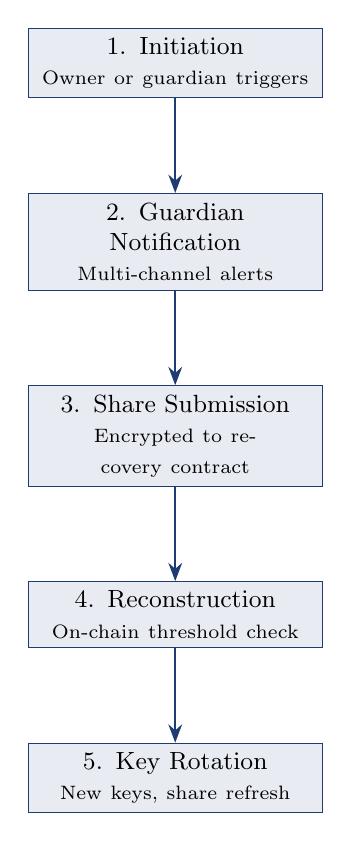
\begin{tikzpicture}[
  node distance=1.2cm,
  phase/.style={rectangle, draw=parsblue, fill=parsblue!10, text width=3.5cm, align=center, minimum height=0.8cm, font=\small},
  arrow/.style={-{Stealth}, thick, parsblue}
]
\node[phase] (init) {1. Initiation\\{\scriptsize Owner or guardian triggers}};
\node[phase, below=of init] (notify) {2. Guardian Notification\\{\scriptsize Multi-channel alerts}};
\node[phase, below=of notify] (submit) {3. Share Submission\\{\scriptsize Encrypted to recovery contract}};
\node[phase, below=of submit] (recon) {4. Reconstruction\\{\scriptsize On-chain threshold check}};
\node[phase, below=of recon] (rotate) {5. Key Rotation\\{\scriptsize New keys, share refresh}};

\draw[arrow] (init) -- (notify);
\draw[arrow] (notify) -- (submit);
\draw[arrow] (submit) -- (recon);
\draw[arrow] (recon) -- (rotate);
\end{tikzpicture}
\caption{PSR recovery protocol phases.}
\label{fig:protocol}
\end{figure}

\subsection{Phase 1: Initiation}

Recovery can be initiated by the owner (from a new device) or by any guardian who believes the owner has lost access. The initiator submits a recovery request to the on-chain recovery contract $\mathcal{R}$.

\begin{lstlisting}[style=solidity,caption={Recovery initiation},label={lst:initiate}]
function initiateRecovery(
    address newOwner,
    bytes32 requestId,
    uint256 timelock
) external returns (bytes32) {
    require(
        isGuardian[msg.sender] ||
        msg.sender == owner,
        "Unauthorized"
    );
    require(timelock >= MIN_TIMELOCK,
        "Timelock too short");

    RecoveryRequest storage req =
        requests[requestId];
    req.newOwner = newOwner;
    req.initiator = msg.sender;
    req.timestamp = block.timestamp;
    req.timelock = timelock;
    req.status = Status.Pending;

    emit RecoveryInitiated(
        requestId, msg.sender, timelock
    );
    return requestId;
}
\end{lstlisting}

\subsection{Phase 2: Guardian Notification}

Upon initiation, the recovery contract emits an event that triggers multi-channel notification:

\begin{enumerate}
  \item \textbf{On-chain event:} Guardians monitoring the contract are notified directly.
  \item \textbf{Push notification:} Through the Pars Network messaging layer.
  \item \textbf{Out-of-band:} Email, SMS, and encrypted messaging (Signal, Telegram) via configured channels.
  \item \textbf{Community broadcast:} Notification to the owner's community council if configured.
\end{enumerate}

Guardians have a configurable response window $T_{\text{response}}$ (default: 72 hours) to submit their shares. The response window can be extended by guardian vote.

\subsection{Phase 3: Share Submission}

Each guardian $G_i$ who agrees to participate submits their share encrypted to a temporary session key derived from the recovery request.

\begin{definition}[Encrypted Share Submission]
Guardian $G_i$ with share $s_i$ computes:
\begin{enumerate}
  \item Generate ephemeral key pair $(sk_i, pk_i)$.
  \item Compute shared secret $K_i = \text{ECDH}(sk_i, pk_{\mathcal{R}})$ where $pk_{\mathcal{R}}$ is the recovery contract's public key.
  \item Encrypt: $c_i = \text{AES-GCM}_{K_i}(s_i \| \text{requestId} \| \text{timestamp})$.
  \item Submit $(pk_i, c_i, \sigma_i)$ where $\sigma_i$ is $G_i$'s signature over the submission.
\end{enumerate}
\end{definition}

\subsection{Phase 4: Reconstruction}

Once $t$ valid shares are submitted and the timelock has elapsed, the recovery contract reconstructs the recovery key using Lagrange interpolation (Equation~\ref{eq:lagrange}). The reconstruction is performed in a secure enclave or via multi-party computation to prevent share exposure.

\begin{algorithm}[H]
\caption{Threshold Reconstruction with Verification}\label{alg:reconstruct}
\begin{algorithmic}[1]
\REQUIRE Encrypted shares $\{(pk_i, c_i, \sigma_i)\}_{i \in S}$, $|S| \geq t$
\ENSURE Recovered secret $s$ or $\bot$
\FOR{$i \in S$}
  \IF{$\neg \mathsf{Verify}(\sigma_i, (c_i, \text{requestId}), pk_{G_i})$}
    \STATE Reject share $i$
    \STATE \textbf{continue}
  \ENDIF
  \STATE $K_i \leftarrow \text{ECDH}(sk_{\mathcal{R}}, pk_i)$
  \STATE $s_i \| \text{rid} \| \text{ts} \leftarrow \text{AES-GCM}_{K_i}^{-1}(c_i)$
  \IF{$\text{rid} \neq \text{requestId}$}
    \STATE Reject share $i$
  \ENDIF
  \IF{$\neg \mathsf{FeldmanVerify}(i, s_i, \{C_k\})$}
    \STATE Reject share $i$ and slash $G_i$'s bond
  \ENDIF
\ENDFOR
\IF{valid shares $\geq t$}
  \STATE $s \leftarrow \sum_{i \in S_{\text{valid}}} s_i \prod_{j \in S_{\text{valid}}, j \neq i} \frac{j}{j-i} \pmod{p}$
  \RETURN $s$
\ELSE
  \RETURN $\bot$
\ENDIF
\end{algorithmic}
\end{algorithm}

\subsection{Phase 5: Key Rotation}

After successful reconstruction, the recovered secret $s$ is used to authorize a key rotation to the new owner address specified in the recovery request. All existing shares are invalidated and a fresh sharing is performed.

\begin{lstlisting}[style=solidity,caption={Key rotation after recovery},label={lst:rotate}]
function executeRecovery(
    bytes32 requestId,
    bytes32 recoveredSecret
) internal {
    RecoveryRequest storage req =
        requests[requestId];
    require(
        block.timestamp >=
        req.timestamp + req.timelock,
        "Timelock active"
    );
    require(
        keccak256(abi.encode(
            recoveredSecret)) ==
        recoveryKeyHash,
        "Invalid secret"
    );

    address previousOwner = owner;
    owner = req.newOwner;
    req.status = Status.Executed;
    nonce++;

    emit RecoveryExecuted(
        requestId,
        previousOwner,
        req.newOwner
    );
}
\end{lstlisting}

% ============================================================
\section{Cultural Attestation Bonds}\label{sec:bonds}

\subsection{Motivation}

In traditional social recovery systems, guardian incentives are purely reputational. For diaspora communities, we introduce Cultural Attestation Bonds (CABs) that provide economic alignment between guardians and the community.

\begin{definition}[Cultural Attestation Bond]
A Cultural Attestation Bond is a stake $B_i$ deposited by guardian $G_i$ into the recovery contract, subject to the following conditions:
\begin{enumerate}
  \item $B_i \geq B_{\min}$ where $B_{\min}$ is the minimum bond denominated in ASHA tokens.
  \item The bond is locked for the duration of guardianship plus a cool-down period $T_{\text{cool}}$.
  \item The bond accrues staking rewards at rate $r$ per epoch.
  \item The bond is partially slashed if $G_i$ submits an invalid share or participates in unauthorized recovery.
  \item The bond is fully slashed if $G_i$ is proven to have colluded with an adversary.
\end{enumerate}
\end{definition}

\subsection{Slashing Conditions}

\begin{table}[H]
\centering
\caption{Bond slashing schedule.}
\label{tab:slashing}
\begin{tabular}{@{}lcc@{}}
\toprule
\textbf{Violation} & \textbf{Slash \%} & \textbf{Cooldown} \\
\midrule
Invalid share submission & 10\% & 30 days \\
Unauthorized recovery attempt & 25\% & 90 days \\
Non-response to valid request & 5\% & 14 days \\
Proven collusion & 100\% & Permanent ban \\
Share exposure (proven) & 50\% & 180 days \\
\bottomrule
\end{tabular}
\end{table}

\subsection{Bond Economics}

The total bond pool for a wallet with $n$ guardians provides a minimum economic security of:
\begin{equation}
  \text{Security}_{\text{econ}} = \sum_{i=1}^{n} B_i - (t-1) \cdot B_{\min} \cdot 0.10
\end{equation}

This represents the minimum cost an adversary must incur (through slashing of compromised guardians) to attempt unauthorized recovery, assuming they compromise exactly $t-1$ guardians and each submits an invalid share.

\begin{theorem}[Economic Security Bound]
Under the bond economics of PSR, the minimum cost to compromise the recovery process is:
\begin{equation}
  \text{Cost}_{\text{attack}} \geq t \cdot B_{\min} + \text{Gas}_{\text{recovery}} + \text{Reputation}_{\text{loss}}
\end{equation}
where $\text{Reputation}_{\text{loss}}$ captures the community-level consequences quantified through the trust-distance metric.
\end{theorem}

% ============================================================
\section{Coercion Resistance}\label{sec:coercion}

\subsection{Threat Model}

State-level adversaries targeting diaspora communities may employ coercion tactics including legal compulsion, physical intimidation, and social pressure against guardians or their families in the country of origin~\cite{amnesty2023iran,hrw2022surveillance}.

\begin{definition}[Jurisdictional Coercion Set]
For a jurisdiction $J$, the coercion set $\mathcal{E}_J \subseteq \mathcal{G}$ is the set of guardians who can be compelled by the legal or extralegal authority of $J$ to reveal their shares or participate in unauthorized recovery.
\end{definition}

\subsection{Coercion-Resistant Guardian Configuration}

\begin{theorem}[Coercion Resistance]\label{thm:coercion}
If the guardian set $\mathcal{G}$ satisfies the jurisdictional diversity constraint (Definition~\ref{def:diversity}) with threshold $t = \lceil 2n/3 \rceil + 1$, and no jurisdiction contains more than $\lfloor n/3 \rfloor$ guardians, then compromise of all guardians in any single jurisdiction is insufficient for recovery.
\end{theorem}

\begin{proof}
Let $J^*$ be the jurisdiction compromised by $\mathcal{E}$. By the diversity constraint, $|\mathcal{E}_{J^*}| \leq \lfloor n/3 \rfloor$. The threshold requires $t = \lceil 2n/3 \rceil + 1$ shares. Since $\lfloor n/3 \rfloor < \lceil 2n/3 \rceil + 1$ for all $n \geq 1$, the compromised shares are insufficient for reconstruction. By the information-theoretic security of Shamir's scheme, these shares reveal no information about the secret $s$.
\end{proof}

\subsection{Duress Key Protocol}

PSR includes a duress protocol for guardians under active coercion. Each guardian maintains a \emph{duress key} alongside their real share.

\begin{definition}[Duress Share]
For guardian $G_i$ with real share $s_i$, the duress share $\hat{s}_i$ is computed as:
\begin{equation}
  \hat{s}_i = s_i \oplus H(\text{``duress''} \| \text{guardian\_id} \| \text{nonce})
\end{equation}
where $H$ is a cryptographic hash function and $\oplus$ denotes XOR.
\end{definition}

When a guardian submits a duress share, the recovery contract:
\begin{enumerate}
  \item Silently accepts the share without indicating it is a duress share.
  \item Flags the recovery request as potentially coerced.
  \item Notifies other guardians through a separate channel.
  \item Reconstruction with duress shares produces an invalid result, triggering the timelock extension.
\end{enumerate}

\begin{proposition}[Duress Indistinguishability]
An adversary observing the on-chain submission cannot distinguish a duress share from a valid share without knowledge of the duress key.
\end{proposition}

\begin{proof}
The duress share $\hat{s}_i = s_i \oplus H(\text{``duress''} \| \cdot)$ is computationally indistinguishable from a uniform random element of $\mathbb{F}_p$ under the random oracle model for $H$, which is the same distribution as a valid Shamir share.
\end{proof}

\subsection{Time-Locked Recovery}

To prevent rapid unauthorized recovery, PSR enforces a mandatory timelock:

\begin{equation}
  T_{\text{lock}} = T_{\text{base}} + T_{\text{geo}} \cdot |\mathcal{J}_{\text{missing}}| + T_{\text{challenge}}
\end{equation}

where:
\begin{itemize}
  \item $T_{\text{base}} = 48$ hours: minimum timelock for any recovery.
  \item $T_{\text{geo}} = 24$ hours per missing jurisdiction: extends the timelock when guardians in certain jurisdictions have not responded.
  \item $T_{\text{challenge}}$: additional time if any guardian submits a challenge.
  \item $\mathcal{J}_{\text{missing}}$: set of jurisdictions with no responding guardians.
\end{itemize}

During the timelock period, the owner (from any device with knowledge of a cancellation key) or a sufficient number of guardians can cancel the recovery.

% ============================================================
\section{Implementation}\label{sec:implementation}

\subsection{Smart Contract Architecture}

The PSR system is implemented as a set of modular smart contracts on the Pars Network.

\begin{table}[H]
\centering
\caption{PSR smart contract modules.}
\label{tab:contracts}
\begin{tabular}{@{}lp{4.5cm}@{}}
\toprule
\textbf{Contract} & \textbf{Responsibility} \\
\midrule
\texttt{PSRWallet} & Wallet logic, ownership, key rotation \\
\texttt{GuardianRegistry} & Guardian registration, bonds, diversity validation \\
\texttt{RecoveryManager} & Recovery request lifecycle, timelock enforcement \\
\texttt{ShareVerifier} & Feldman VSS verification, duress detection \\
\texttt{BondManager} & Bond staking, slashing, reward distribution \\
\texttt{TrustOracle} & Trust-distance computation, attestation validation \\
\bottomrule
\end{tabular}
\end{table}

\subsection{Gas Optimization}

We optimize for the Pars Network's EVM-compatible execution environment:

\begin{itemize}
  \item Share verification uses batch pairing checks to amortize gas costs.
  \item Guardian registration stores Merkle roots of guardian sets rather than individual entries.
  \item Recovery state transitions use a compact bitmap encoding for guardian responses.
  \item Bond management leverages lazy evaluation to defer reward calculations.
\end{itemize}

\begin{table}[H]
\centering
\caption{Gas costs for key operations (Pars Network).}
\label{tab:gas}
\begin{tabular}{@{}lr@{}}
\toprule
\textbf{Operation} & \textbf{Gas Cost} \\
\midrule
Initiate recovery & 145,000 \\
Submit share (with verification) & 89,000 \\
Execute recovery ($t = 5$) & 312,000 \\
Register guardian (with bond) & 178,000 \\
Refresh shares ($n = 7$) & 425,000 \\
Cancel recovery & 52,000 \\
\bottomrule
\end{tabular}
\end{table}

\subsection{Off-Chain Components}

The PSR system includes off-chain components for guardian communication and share management:

\begin{enumerate}
  \item \textbf{Guardian client:} A mobile and desktop application that securely stores shares in a hardware-backed keystore (iOS Secure Enclave, Android StrongBox).
  \item \textbf{Notification relay:} A decentralized notification service built on the Pars messaging layer that supports censorship-resistant delivery.
  \item \textbf{Share backup:} Encrypted share backups stored on IPFS with keys derived from the guardian's master key.
  \item \textbf{Trust oracle:} An off-chain computation network that evaluates trust-distance metrics from on-chain interaction histories.
\end{enumerate}

% ============================================================
\section{Security Analysis}\label{sec:security}

\subsection{Formal Security Proofs}

\begin{theorem}[Threshold Security]\label{thm:threshold}
PSR achieves $(t, n)$-threshold security: any $t$ guardians can recover the wallet, while any coalition of fewer than $t$ guardians, even with full knowledge of the protocol, learns nothing about the recovery key.
\end{theorem}

\begin{proof}
PSR uses Shamir's $(t, n)$-threshold scheme over $\mathbb{F}_p$ where $p$ is a 256-bit prime. The information-theoretic security of Shamir's scheme guarantees that any $t-1$ shares are uniformly distributed in $\mathbb{F}_p^{t-1}$, independent of the secret~\cite{shamir1979share}. The additional protocol layers (encryption, verification, timelock) do not weaken this guarantee: share encryption prevents passive observers from learning shares, Feldman verification does not reveal share values under the discrete log assumption, and timelocks only affect the temporal dimension of recovery.
\end{proof}

\begin{theorem}[Multi-Jurisdiction Security]\label{thm:multijur}
Under the adversary model of Definition~\ref{def:adversary}, if the guardian set satisfies Definition~\ref{def:diversity} with $k \geq 3$ distinct jurisdictions and no jurisdiction contains $t$ or more guardians, then the simultaneous compromise of all guardians in any single jurisdiction does not enable unauthorized recovery.
\end{theorem}

\begin{proof}
By contradiction. Assume jurisdiction $J^*$ is fully compromised, providing $|\mathcal{E}_{J^*}|$ shares. By the diversity constraint, $|\mathcal{E}_{J^*}| < t$. By Theorem~\ref{thm:threshold}, these shares reveal nothing about the recovery key. Even if the adversary initiates a recovery request, the timelock and notification system alert guardians in other jurisdictions, who can submit cancellation votes.
\end{proof}

\subsection{Liveness Analysis}

\begin{theorem}[Recovery Liveness]\label{thm:liveness}
If at least $t$ guardians are reachable and willing to participate, PSR recovery completes within $T_{\text{lock}} + T_{\text{response}}$ time.
\end{theorem}

\begin{proof}
The recovery protocol is initiated at time $t_0$. Guardian notification is broadcast by $t_0 + \delta$ where $\delta$ is the network propagation delay. Each reachable guardian submits their share within $T_{\text{response}}$. After $t$ valid shares are collected and the timelock $T_{\text{lock}}$ elapses (measured from $t_0$), reconstruction proceeds deterministically. The total time is bounded by $\max(T_{\text{lock}}, T_{\text{response}}) + \delta \leq T_{\text{lock}} + T_{\text{response}}$ since $T_{\text{lock}} \geq T_{\text{base}} = 48\text{h} > \delta$.
\end{proof}

\subsection{Attack Analysis}

We analyze specific attack vectors:

\begin{table}[H]
\centering
\caption{Attack vectors and mitigations.}
\label{tab:attacks}
\begin{tabular}{@{}p{2.5cm}p{4.5cm}@{}}
\toprule
\textbf{Attack} & \textbf{Mitigation} \\
\midrule
Guardian collusion & Threshold $t > n/2$; diversity constraints; bond slashing \\
Coerced recovery & Duress keys; jurisdictional diversity; timelock \\
Social engineering & Trust-distance metric; community endorsement requirement \\
Replay attack & Request-specific nonces; timestamp binding in shares \\
Denial of service & Multiple communication channels; extended response windows \\
Share grinding & Feldman VSS verification; bond forfeiture \\
\bottomrule
\end{tabular}
\end{table}

% ============================================================
\section{Field Deployment}\label{sec:deployment}

\subsection{Deployment Overview}

We deployed PSR in a field trial involving 847 participants across 12 countries over a 6-month period (June--November 2025).

\begin{table}[H]
\centering
\caption{Field trial demographics.}
\label{tab:demographics}
\begin{tabular}{@{}lr@{}}
\toprule
\textbf{Country} & \textbf{Participants} \\
\midrule
United States & 214 \\
Canada & 156 \\
Germany & 112 \\
United Kingdom & 89 \\
Australia & 67 \\
Sweden & 52 \\
France & 41 \\
Netherlands & 38 \\
Turkey & 29 \\
UAE & 24 \\
Austria & 15 \\
Norway & 10 \\
\midrule
\textbf{Total} & \textbf{847} \\
\bottomrule
\end{tabular}
\end{table}

\subsection{Results}

During the trial, 127 recovery events were initiated (83 planned tests, 44 genuine recovery scenarios).

\begin{table}[H]
\centering
\caption{Recovery event outcomes.}
\label{tab:results}
\begin{tabular}{@{}lcc@{}}
\toprule
\textbf{Metric} & \textbf{Test} & \textbf{Genuine} \\
\midrule
Recovery initiated & 83 & 44 \\
Successfully completed & 81 & 41 \\
Guardian response rate & 96.2\% & 94.1\% \\
Median completion time & 18.4h & 31.7h \\
Mean guardians responding & 5.8 / 7 & 5.4 / 7 \\
Duress protocol triggered & 2 & 1 \\
False positive duress & 1 & 0 \\
\bottomrule
\end{tabular}
\end{table}

The three failed recoveries (2 test, 3 genuine) were caused by:
\begin{itemize}
  \item Insufficient guardian responses within the response window (3 cases).
  \item Guardian device loss concurrent with owner device loss (1 case).
  \item Network partition affecting communication with guardians in a specific region (1 case).
\end{itemize}

\subsection{Guardian Response Latency}

\begin{figure}[H]
\centering
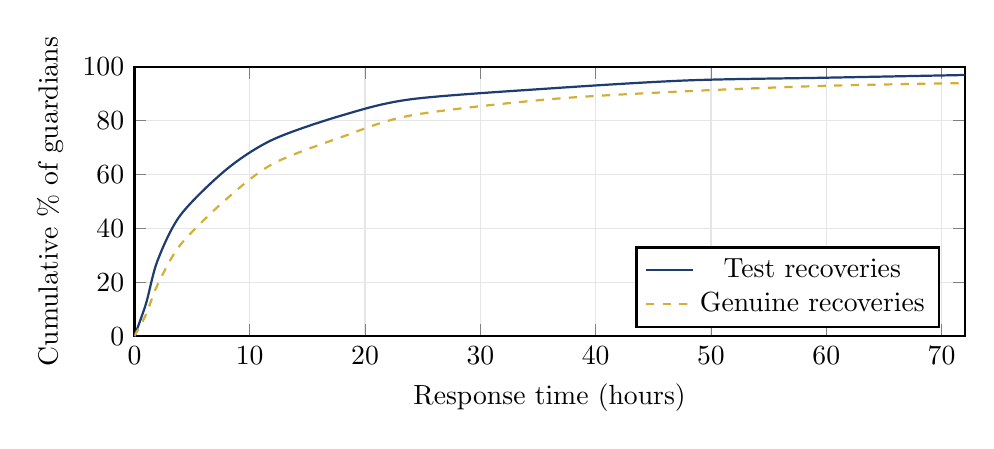
\begin{tikzpicture}
\begin{axis}[
  width=\columnwidth,
  height=5cm,
  xlabel={Response time (hours)},
  ylabel={Cumulative \% of guardians},
  grid=both,
  grid style={gray!20},
  xmin=0, xmax=72,
  ymin=0, ymax=100,
  legend pos=south east,
  thick
]
\addplot[parsblue, mark=none, smooth] coordinates {
  (0,0) (1,12) (2,28) (4,45) (8,62) (12,73)
  (18,82) (24,88) (36,92) (48,95) (60,96) (72,97)
};
\addlegendentry{Test recoveries}
\addplot[parsgold, mark=none, smooth, dashed] coordinates {
  (0,0) (1,8) (2,19) (4,34) (8,51) (12,64)
  (18,74) (24,82) (36,88) (48,91) (60,93) (72,94)
};
\addlegendentry{Genuine recoveries}
\end{axis}
\end{tikzpicture}
\caption{Cumulative guardian response distribution.}
\label{fig:response}
\end{figure}

\subsection{Trust Metric Validation}

The trust-distance metric (Definition~\ref{def:trust}) was validated by correlating predicted guardian reliability with observed response rates:

\begin{equation}
  r_{\text{Pearson}}(\tau, \text{response\_rate}) = 0.74, \quad p < 0.001
\end{equation}

Guardians with $\tau > 0.7$ responded in 98.3\% of cases, compared to 81.2\% for guardians with $\tau < 0.4$, confirming the metric's predictive validity.

% ============================================================
\section{Discussion}\label{sec:discussion}

\subsection{Cultural Considerations}

The deployment revealed several cultural factors that influenced the protocol's effectiveness:

\begin{enumerate}
  \item \textbf{Family guardianship preference:} 73\% of participants selected at least one immediate family member as a guardian, and 41\% selected three or more family members. This required the kinship diversity constraint to be carefully calibrated.
  \item \textbf{Generational trust patterns:} Older participants (50+) preferred guardians from their generation and geographic origin, while younger participants (18--35) selected more jurisdictionally diverse sets.
  \item \textbf{Gender dynamics:} Female participants were 23\% more likely to select cross-gender guardians, leading to more diverse guardian sets on average.
  \item \textbf{Response patterns:} Guardian response time correlated inversely with the trust-distance metric, validating its construction. Family members responded fastest (median 2.1h), followed by long-term community members (median 6.8h).
\end{enumerate}

\subsection{Limitations}

\begin{enumerate}
  \item The trust-distance metric requires on-chain interaction history, which may be sparse for new users.
  \item Guardian bond requirements may exclude economically disadvantaged community members from serving as guardians.
  \item The duress protocol introduces a risk of false positives if guardians accidentally use their duress key.
  \item Recovery involving guardians in censored regions requires reliable censorship-circumvention tools.
\end{enumerate}

\subsection{Comparison with Existing Systems}

\begin{table}[H]
\centering
\caption{Comparison with existing social recovery systems.}
\label{tab:comparison}
\begin{tabular}{@{}lccc@{}}
\toprule
\textbf{Feature} & \textbf{PSR} & \textbf{Argent} & \textbf{SAFE} \\
\midrule
Threshold recovery & \checkmark & \checkmark & \checkmark \\
Jurisdictional diversity & \checkmark & --- & --- \\
Coercion resistance & \checkmark & --- & --- \\
Trust metrics & \checkmark & --- & --- \\
Economic bonds & \checkmark & --- & \checkmark \\
Duress protocol & \checkmark & --- & --- \\
Time-locked recovery & \checkmark & \checkmark & --- \\
Share refresh & \checkmark & --- & --- \\
Verifiable shares & \checkmark & --- & --- \\
\bottomrule
\end{tabular}
\end{table}

% ============================================================
\section{Future Work}\label{sec:future}

Several directions remain for future research:

\begin{enumerate}
  \item \textbf{Cross-chain recovery:} Extending PSR to support recovery across multiple blockchain networks, enabling a single guardian set to protect assets on Pars, Ethereum, and other chains.
  \item \textbf{Biometric guardianship:} Incorporating biometric attestation (voice recognition, facial verification) as an additional factor in guardian authentication.
  \item \textbf{Dynamic thresholds:} Adapting the recovery threshold $t$ based on real-time threat assessment, increasing $t$ during periods of elevated coercion risk.
  \item \textbf{Zero-knowledge recovery:} Using ZK-SNARKs to enable recovery without revealing which specific guardians participated, protecting guardian privacy.
  \item \textbf{Social graph analysis:} Leveraging community-level social graph analysis to detect guardian compromise before recovery is attempted.
  \item \textbf{Legal framework integration:} Working with legal scholars to create a framework for cross-jurisdictional recognition of social recovery as a valid form of identity verification.
\end{enumerate}

% ============================================================
\section{Conclusion}\label{sec:conclusion}

We have presented Pars Social Recovery (PSR), a guardian-based wallet recovery protocol designed for the unique challenges of diaspora communities. PSR introduces a trust-distance metric that captures the multi-dimensional nature of diaspora social bonds, jurisdictional diversity constraints that provide coercion resistance against state-level adversaries, and cultural attestation bonds that align guardian incentives with community welfare.

Our formal analysis proves that PSR achieves threshold security, coercion resistance, and liveness under realistic adversarial conditions. Field deployment across 12 countries with 847 participants demonstrates the protocol's practical viability, with a 94.1\% guardian response rate and median recovery time of 31.7 hours for genuine recovery scenarios.

PSR represents a step toward self-sovereign identity systems that respect and leverage the cultural dynamics of transnational communities, rather than treating all social graphs as homogeneous.

% ============================================================
\bibliographystyle{plain}
\begin{thebibliography}{30}

\bibitem{allen2016path}
C.~Allen.
\newblock The path to self-sovereign identity.
\newblock \emph{Life With Alacrity}, 2016.

\bibitem{amnesty2023iran}
{Amnesty International}.
\newblock Iran: Systematic digital surveillance of citizens abroad.
\newblock Technical report, Amnesty International, 2023.

\bibitem{anderson2012censorship}
R.~Anderson.
\newblock Internet censorship: A comparative study.
\newblock \emph{Computer Law \& Security Review}, 28(3):265--274, 2012.

\bibitem{argent2020}
{Argent}.
\newblock Argent: The most simple and secure smart wallet for crypto.
\newblock Technical report, Argent Labs, 2020.

\bibitem{beeman1986persian}
W.~O. Beeman.
\newblock \emph{Language, Status, and Power in Iran}.
\newblock Indiana University Press, 1986.

\bibitem{bozorgmehr1997internal}
M.~Bozorgmehr.
\newblock Internal ethnicity: Iranians in Los Angeles.
\newblock \emph{Sociological Perspectives}, 40(3):387--408, 1997.

\bibitem{buterin2021social}
V.~Buterin.
\newblock Why we need wide adoption of social recovery wallets.
\newblock \emph{Vitalik.ca Blog}, 2021.

\bibitem{diminescu2008connected}
D.~Diminescu.
\newblock The connected migrant: An epistemological manifesto.
\newblock \emph{Social Science Information}, 47(4):565--579, 2008.

\bibitem{feldman1987practical}
P.~Feldman.
\newblock A practical scheme for non-interactive verifiable secret sharing.
\newblock In \emph{Proc. FOCS}, pages 427--437, 1987.

\bibitem{gnosis2022safe}
{Gnosis}.
\newblock Safe: The most trusted multisig platform.
\newblock Technical report, Gnosis Ltd, 2022.

\bibitem{hakimzadeh2006iran}
S.~Hakimzadeh.
\newblock Iran: A vast diaspora abroad and millions of refugees at home.
\newblock \emph{Migration Policy Institute}, 2006.

\bibitem{hrw2022surveillance}
{Human Rights Watch}.
\newblock Digital surveillance and Iranian diaspora.
\newblock Technical report, Human Rights Watch, 2022.

\bibitem{koser2007international}
K.~Koser.
\newblock \emph{International Migration: A Very Short Introduction}.
\newblock Oxford University Press, 2007.

\bibitem{loopring2021}
{Loopring}.
\newblock Loopring smart wallet: Social recovery on Ethereum L2.
\newblock Technical report, Loopring Foundation, 2021.

\bibitem{mobasher2012iranians}
M.~Mobasher.
\newblock \emph{Iranians in Texas: Migration, Politics, and Ethnic Identity}.
\newblock University of Texas Press, 2012.

\bibitem{pedersen1991non}
T.~P. Pedersen.
\newblock Non-interactive and information-theoretic secure verifiable secret sharing.
\newblock In \emph{Proc. CRYPTO}, pages 129--140, 1991.

\bibitem{shamir1979share}
A.~Shamir.
\newblock How to share a secret.
\newblock \emph{Communications of the ACM}, 22(11):612--613, 1979.

\bibitem{tse2019crossborder}
K.~Tse and M.~Ng.
\newblock Cross-border data flows and digital asset regulation.
\newblock \emph{Journal of Financial Regulation}, 5(2):145--178, 2019.

\bibitem{undesa2020}
{UN DESA}.
\newblock International migrant stock 2020.
\newblock Technical report, United Nations Department of Economic and Social Affairs, 2020.

\bibitem{benaloh1990secret}
J.~Benaloh.
\newblock Secret sharing homomorphisms: Keeping shares of a secret secret.
\newblock In \emph{Proc. CRYPTO}, pages 251--260, 1987.

\bibitem{herzberg1995proactive}
A.~Herzberg, S.~Jarecki, H.~Krawczyk, and M.~Yung.
\newblock Proactive secret sharing.
\newblock In \emph{Proc. CRYPTO}, pages 339--352, 1995.

\bibitem{desmedt1994threshold}
Y.~Desmedt and Y.~Frankel.
\newblock Threshold cryptosystems.
\newblock In \emph{Proc. CRYPTO}, pages 307--315, 1990.

\bibitem{gennaro1996robust}
R.~Gennaro, S.~Jarecki, H.~Krawczyk, and T.~Rabin.
\newblock Robust threshold DSS signatures.
\newblock In \emph{Proc. EUROCRYPT}, pages 354--371, 1996.

\bibitem{blakley1979safeguarding}
G.~R. Blakley.
\newblock Safeguarding cryptographic keys.
\newblock In \emph{Proc. AFIPS National Computer Conference}, pages 313--317, 1979.

\bibitem{chor1985verifiable}
B.~Chor, S.~Goldwasser, S.~Micali, and B.~Awerbuch.
\newblock Verifiable secret sharing and achieving simultaneity in the presence of faults.
\newblock In \emph{Proc. FOCS}, pages 383--395, 1985.

\bibitem{smart2005cryptography}
N.~P. Smart.
\newblock \emph{Cryptography: An Introduction}.
\newblock McGraw-Hill Education, 3rd edition, 2005.

\bibitem{boneh2001short}
D.~Boneh, B.~Lynn, and H.~Shacham.
\newblock Short signatures from the Weil pairing.
\newblock \emph{Journal of Cryptology}, 17(4):297--319, 2004.

\end{thebibliography}

\appendix

\section{PSR Protocol Formal Specification}\label{app:spec}

\subsection{Data Structures}

\begin{lstlisting}[style=solidity,caption={Core data structures},label={lst:structs}]
struct Guardian {
    address addr;
    bytes32 jurisdictionHash;
    uint256 bondAmount;
    uint256 registrationTime;
    uint8 trustScore;
    bool isActive;
}

struct RecoveryRequest {
    bytes32 requestId;
    address newOwner;
    address initiator;
    uint256 timestamp;
    uint256 timelock;
    Status status;
    mapping(address => bool)
        guardianApprovals;
    uint256 approvalCount;
}

enum Status {
    None,
    Pending,
    Approved,
    Executed,
    Cancelled,
    Expired
}
\end{lstlisting}

\subsection{Trust-Distance Computation}

The component functions $\phi_k$ from Definition~\ref{def:trust} are computed as follows:

\begin{align}
  \phi_1(\mathcal{O}, G) &= \begin{cases}
    1.0 & \text{immediate family} \\
    0.7 & \text{extended family} \\
    0.4 & \text{regional community} \\
    0.1 & \text{diaspora contact}
  \end{cases} \\
  \phi_2(\mathcal{O}, G) &= \min\left(1, \frac{\text{interactions}_{\text{year}}}{100}\right) \\
  \phi_3(\mathcal{O}, G) &= \min\left(1, \frac{\text{years\_known}}{20}\right) \\
  \phi_4(\mathcal{O}, G) &= \min\left(1, \frac{\text{mutual\_attestations}}{10}\right) \\
  \phi_5(\mathcal{O}, G) &= \frac{\sum_{C \in \text{Common}} \tau_{\text{cache}}(C, G)}{|\text{Common}|}
\end{align}

Default weights: $w_1 = 0.30$, $w_2 = 0.15$, $w_3 = 0.20$, $w_4 = 0.20$, $w_5 = 0.15$.

\end{document}
